\documentclass[margin,line]{res}
\usepackage{hyperref}
\usepackage{url}
%\usepackage{pgfplotstable}
%\usepackage{booktabs}
\usepackage{graphicx}
\oddsidemargin -.5in
\evensidemargin -.5in
\textwidth=6.0in
\itemsep=0in
\parsep=0in
\topmargin=0in
\topskip=0in
 
\newenvironment{list1}{
  \begin{list}{\ding{113}}{%
      \setlength{\itemsep}{0in}
      \setlength{\parsep}{0in} \setlength{\parskip}{0in}
      \setlength{\topsep}{0in} \setlength{\partopsep}{0in}
      \setlength{\leftmargin}{0.17in}}}{\end{list}}
\newenvironment{list2}{
  \begin{list}{$\bullet$}{%
      \setlength{\itemsep}{0in}
      \setlength{\parsep}{0in} \setlength{\parskip}{0in}
      \setlength{\topsep}{0in} \setlength{\partopsep}{0in}
      \setlength{\leftmargin}{0.2in}}}{\end{list}}


    
\begin{document}
\begin{figure}[h]
%\centering
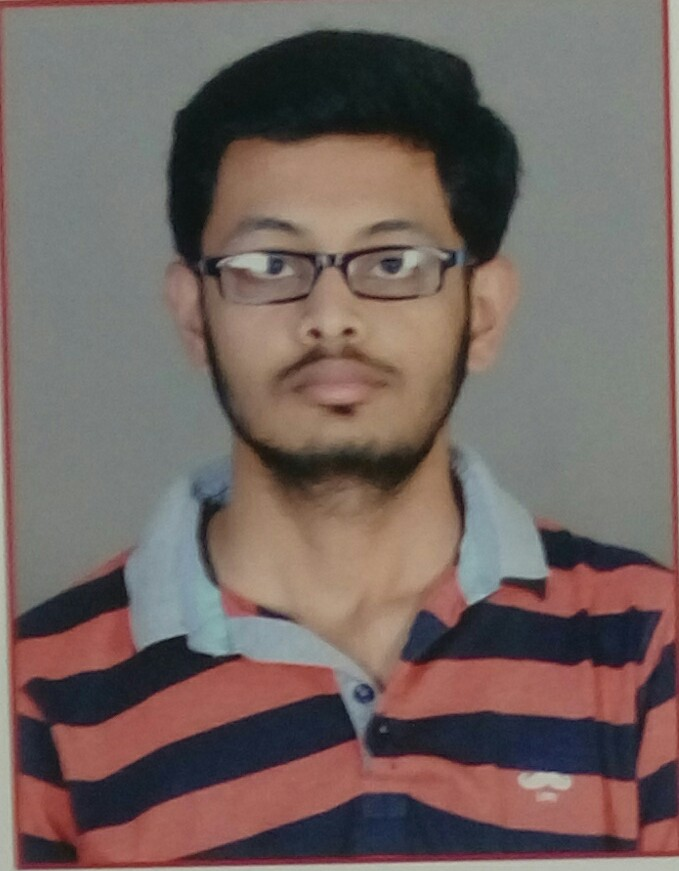
\includegraphics[width=4cm,height=4.5cm]{photo.jpg}
\end{figure}

\name{\huge\ \ \ \ \ \ \ \ \ \ \ \ Bhavy A. Shah} \hfill {\em \today}

\begin{resume}
\section{\sc \bf Contact Information}

\vspace{.05in}
\begin{tabular}{@{}p{3.5in}p{3in}}
3, Sahyog Park-2             & {Mobile No.:}  +917490809177 \\
Opp. Sanjay Pan Corner 
 & {E-mail:}  bhavy414@google.com\\
New Junction Road\\
Surendranagar-363001\\
Gujarat, India\\
\em \url {www.linkedin.com/in/bhavy-shah-6a1687114/}\\
(under updation)
\end{tabular}


\section{\sc \bf Career Objective}

Robotics has been a fantasy world for me since childhood, and growing up with that in mind and later realizing of what it is truely capable of and heights upto which it can take our living globe, I have always tried to improve myself in making its further utilization and trying to enhance my knowledge to make it as much useful as it is possible for it in our life, so as to make my and all living around more worthy and thus keep on tring to innovate life of it.

\section{\sc \bf Personal Info}

D.O.B.: 28/04/1997\\
Father's Name: Ajaypal Shah\\
Mother's Name: Priya Shah\\
Sex: Male\\
Nationality: Indian


\section{\sc \bf Education}
\begin{tabular}{||r|c||}
	\hline
	Degree & B.tech (Mechatronics)\\
	\hline
	College & U.V.Patel College of Engineering\\
	\hline
	University & Ganpat University(Gujarat)\\
	\hline
	Passing Year & 2019\\
	\hline
	GPA(out of 10) & 7.05\\
	\hline
\end{tabular}

\section{\sc \bf Training \& Internships}
\begin{itemize}

\item Uday Industries, Surendranagar, Gujarat (1.5 months)
\item Bosch Rexroth Training Center, Ganpat University, Mehsana, Gujarat
\end{itemize}

\section{\sc \bf Projects}
\begin{enumerate}

\item {\bf Team UVPCE 5.0 --- ABU Robocon 2017}\\
Worked as {\em lead 3D modeller \& Designer} in the teram of 20 members while working for the Nationals of  International competition of ROBOCON 2017.\\
We designed and made a robot mechanism that was to work on the given theme by host country, to throw disks from a certain distance on flat surfaces at specific heights and distances and to have them land on the surface.

\item{\bf Boeing Aeromodelling Competition 2018}\\
We were a team of four members that worked on making of a simplified jet plane design using material styrofoam and participated in this Event. In the team, all the{\em designing and some portion of fabrication} was carried out by myself. Unfortunately, due to electronics failure, we were unable to showcase it at the last moments in the main event.

\item{\bf Team Armanoid --- Gesture designated \& Voice controlled robotic hand using myograph sensors (eyic-2019)}\\
We were a team of four members and we carried out this project for the our final year assessment as well as participated in the eyic-2019. Our team was national finalist for eyic-2019. My job in the team, {\em apart from being team leader, was designing \& 3D modelling}. Also I had my subsidiary role in fabrication and basic electronics requirements.\\
More details regarding this project can be found in this video :\url{https://youtu.be/Pii0wOFBJWE}

\item {\bf Amazon Alexa skills developer}\\
I am currently learning as well as working on building skills for amazon alexa.\\
Till date, I have made three skills which includes one quiz and two regarding quotes being relied by alexa. However, I am still in the initial stage in learning with amazon alexa and aws enviroment.
\end{enumerate}



\section{\sc\bf Achievements}
\begin{itemize}

\item Team UVPCE secured 20th ranking in the ABU Robocon 2017 National competition among 112 teams

\item Team Armanoid was national finalists for the eyic-2019 competition and ranked among top 21 teams from 362 teams
\end{itemize}


\section{\sc \bf Technical Skills}
\begin{itemize}

\item {\bf Programming Languages:} C, C++, Python, Arduino Programming
\item {\bf Softwares skills:} Solidworks {\em (CSWA Certified)}, Multisim Circuit designing
\item {\bf Mechanical Designing:} Robotics Parameter calculations, Electromechanical Systems design \& calculations, Algorithm designing
\item {\bf Other:} Soldering \& Circuit assembling, Fabrication \& Assembling mechanical products, producing basic mechanical components, Technical problem solving 
\end{itemize}

\section{\sc \bf Extra-curricular Activities}
\begin{itemize}

\item Member-- Robocon Club (2016-17)
\item Member-- Aeromodelling Club (2017-18)
\item E-YIC (2018-19)
\item Shodh Innovative Idea Participant (2018-2019)
\item Amazon Alexa Developer

\end{itemize}

\section{\sc \bf Research Publications}

\begin{enumerate}

\item None

\end{enumerate}

\section{\sc \bf Soft Skills}
\begin{enumerate}

\item Leadership
\item Team-work
\item Analytical thinking \& Problem solving
\item Time management
\item Great verbal skills \& Convincing power
\item Hardworking
\item Insomniac working
\item Punctual \& Dedicated
\item Great grasping power

\end{enumerate}



\section{\sc \bf Co-curricular Activities}
\begin{enumerate}

\item 200m Sprinting
\item Sketching
\item Playing Table tennis
\item Writing

\end{enumerate}



\section{\sc \bf References }
Available upon request.

\section{\sc \bf Declaration}

I hereby accept that all the above Infromation is verified by me \& supporting proofs can be produced on demand if required.

\section{\sc \bf Date}

17th April, 2019




\end{resume}
\end{document}




